\section{RESULTADOS EXPERIMENTALES Y DISCUSIÓN}

Los experimentos empíricos se realizaron sobre una muestra estratificada y balanceada de $186,321$ registros del dataset CIC-IoT-2023 ($130,424$ Entrenamiento, $27,948$ Validación y $27,949$ Prueba final).

\subsection{Fase 1: Selección Estadística de Características}
La Figura~\ref{fig:feature_selection} ilustra la jerarquía de importancia de las 15 variables de red con mayor capacidad discriminatoria obtenidas mediante ANOVA F-Test y la métrica de impureza de Gini de Random Forest.

\begin{figure}[H]
\centering
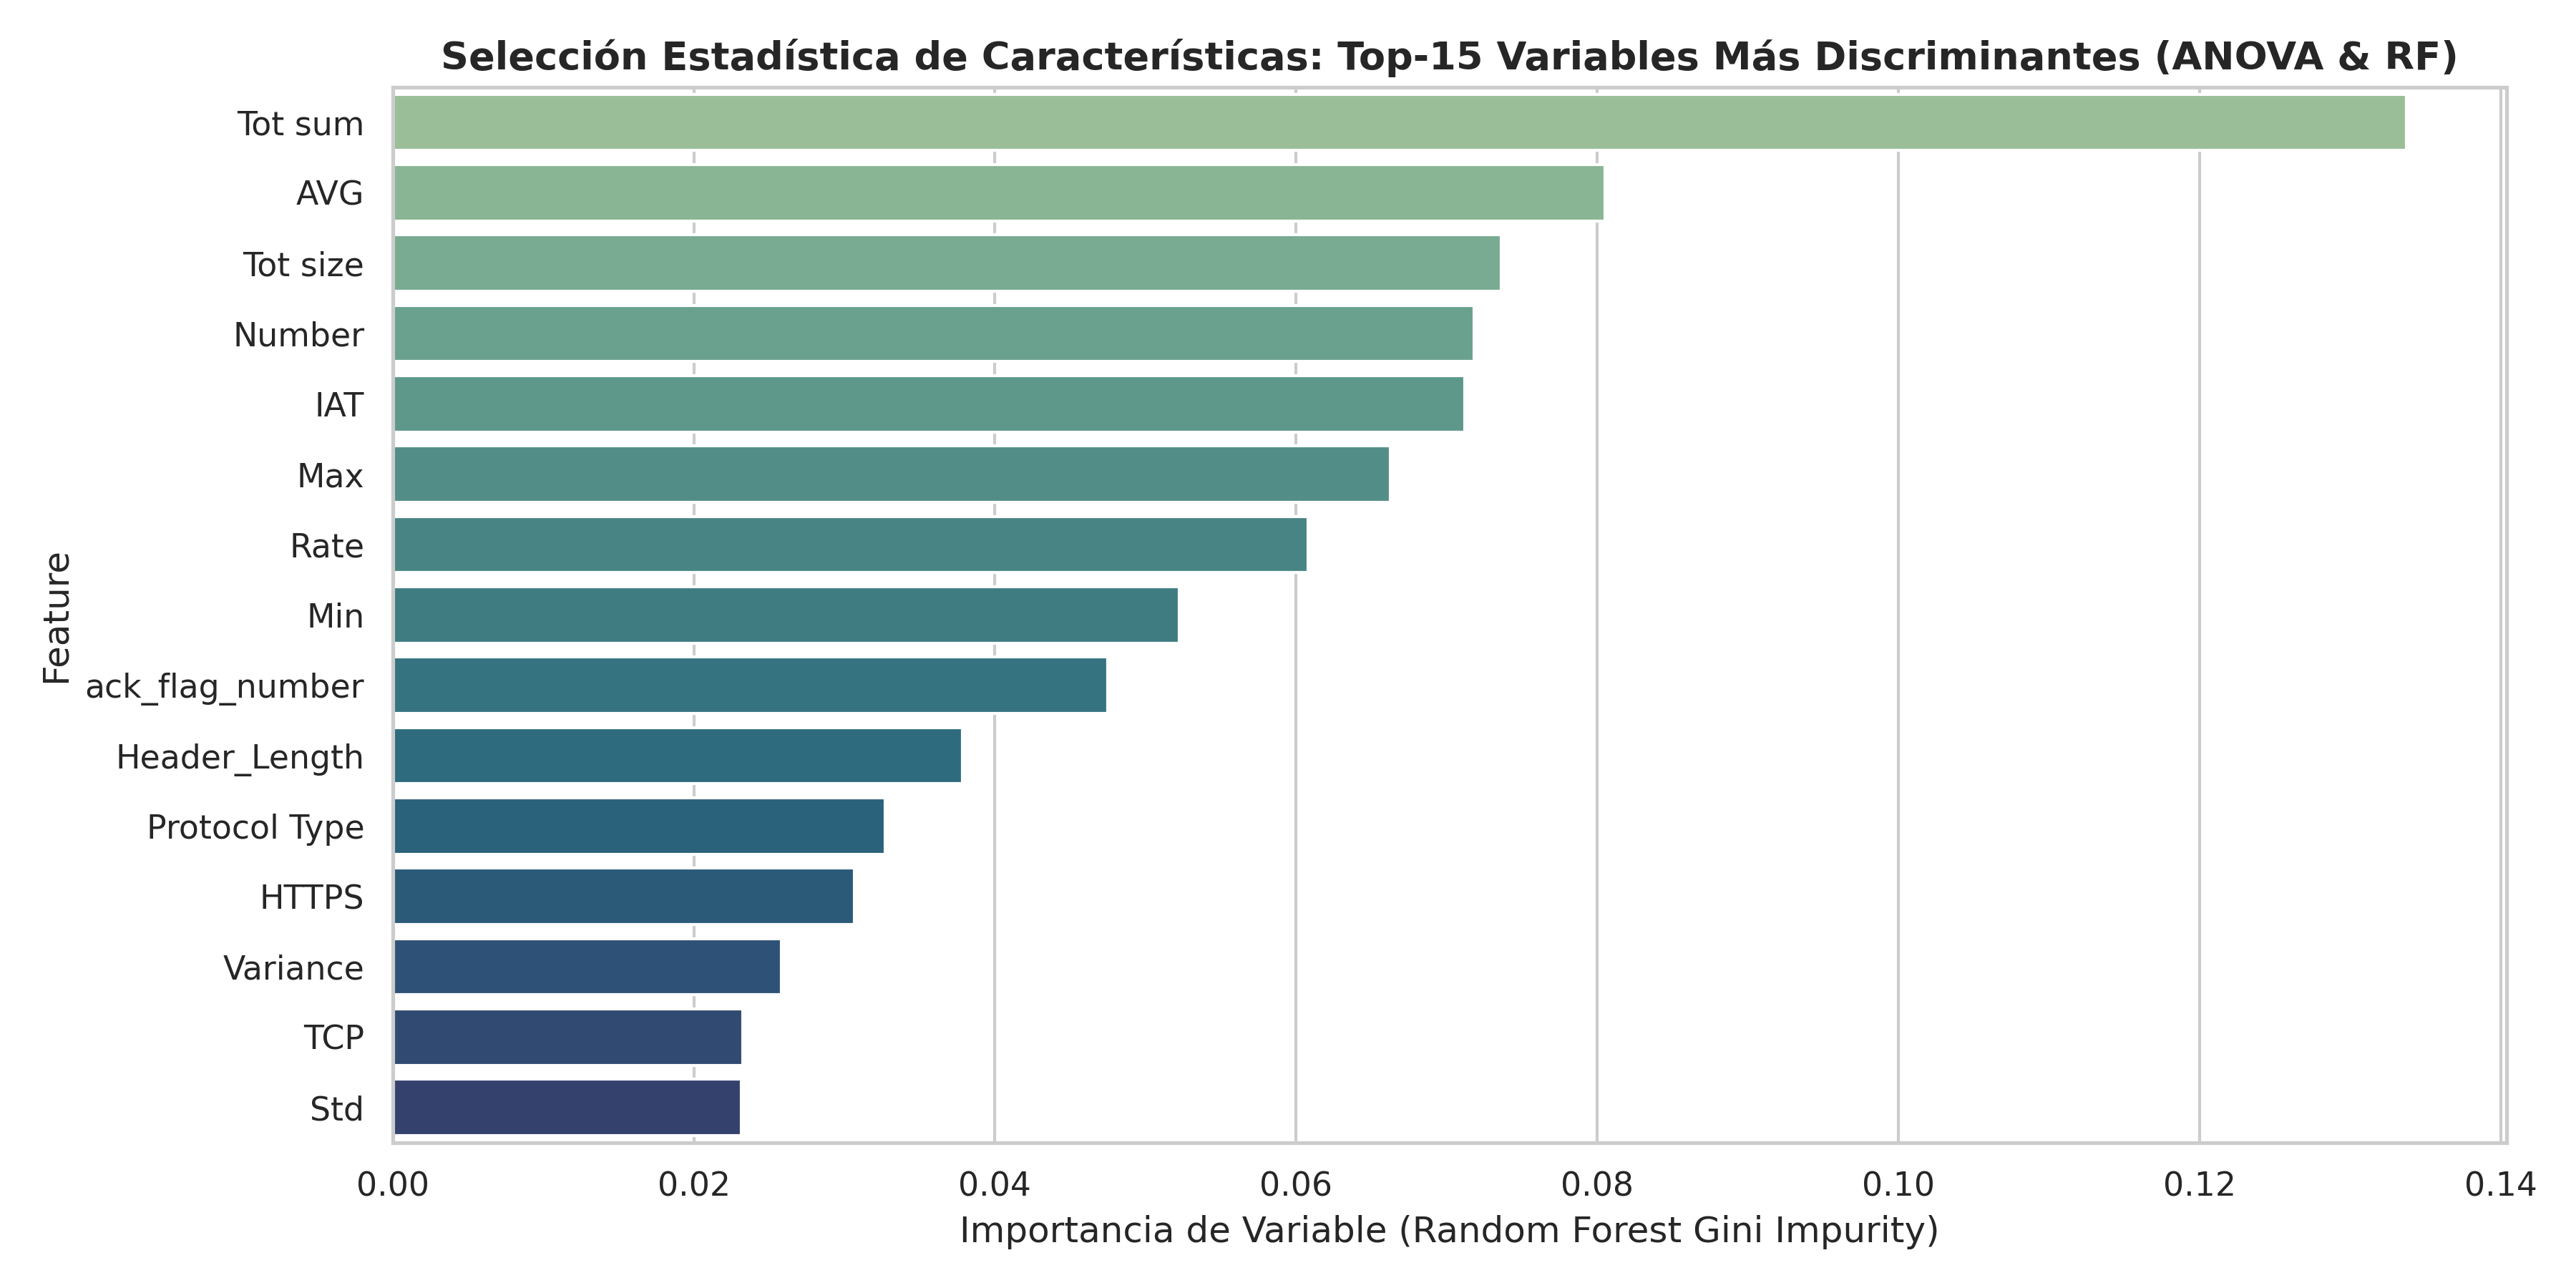
\includegraphics[width=0.92\linewidth]{../results/reports_and_plots/feature_selection_barplot.png}
\caption{Selección Estadística de Características: Top-15 Variables de Red Más Discriminantes.}
\label{fig:feature_selection}
\end{figure}

Variables como \texttt{Header\_Length}, \texttt{Protocol Type}, \texttt{Rate}, \texttt{Tot sum} y \texttt{Tot size} mostraron las puntuaciones $F$ de ANOVA más elevadas, confirmando su rol determinante en la diferenciación de ráfagas DDoS frente a tráfico benigno.

\subsection{Fase 3: Monitoreo de Entrenamiento del VAE-MLP}
La Figura~\ref{fig:training_history} muestra las curvas de evolución de la pérdida combinada ($\mathcal{L}_{\text{total}}$) y la métrica de validación F1-Macro a lo largo de las 40 épocas de entrenamiento en GPU CUDA.

\begin{figure}[H]
\centering
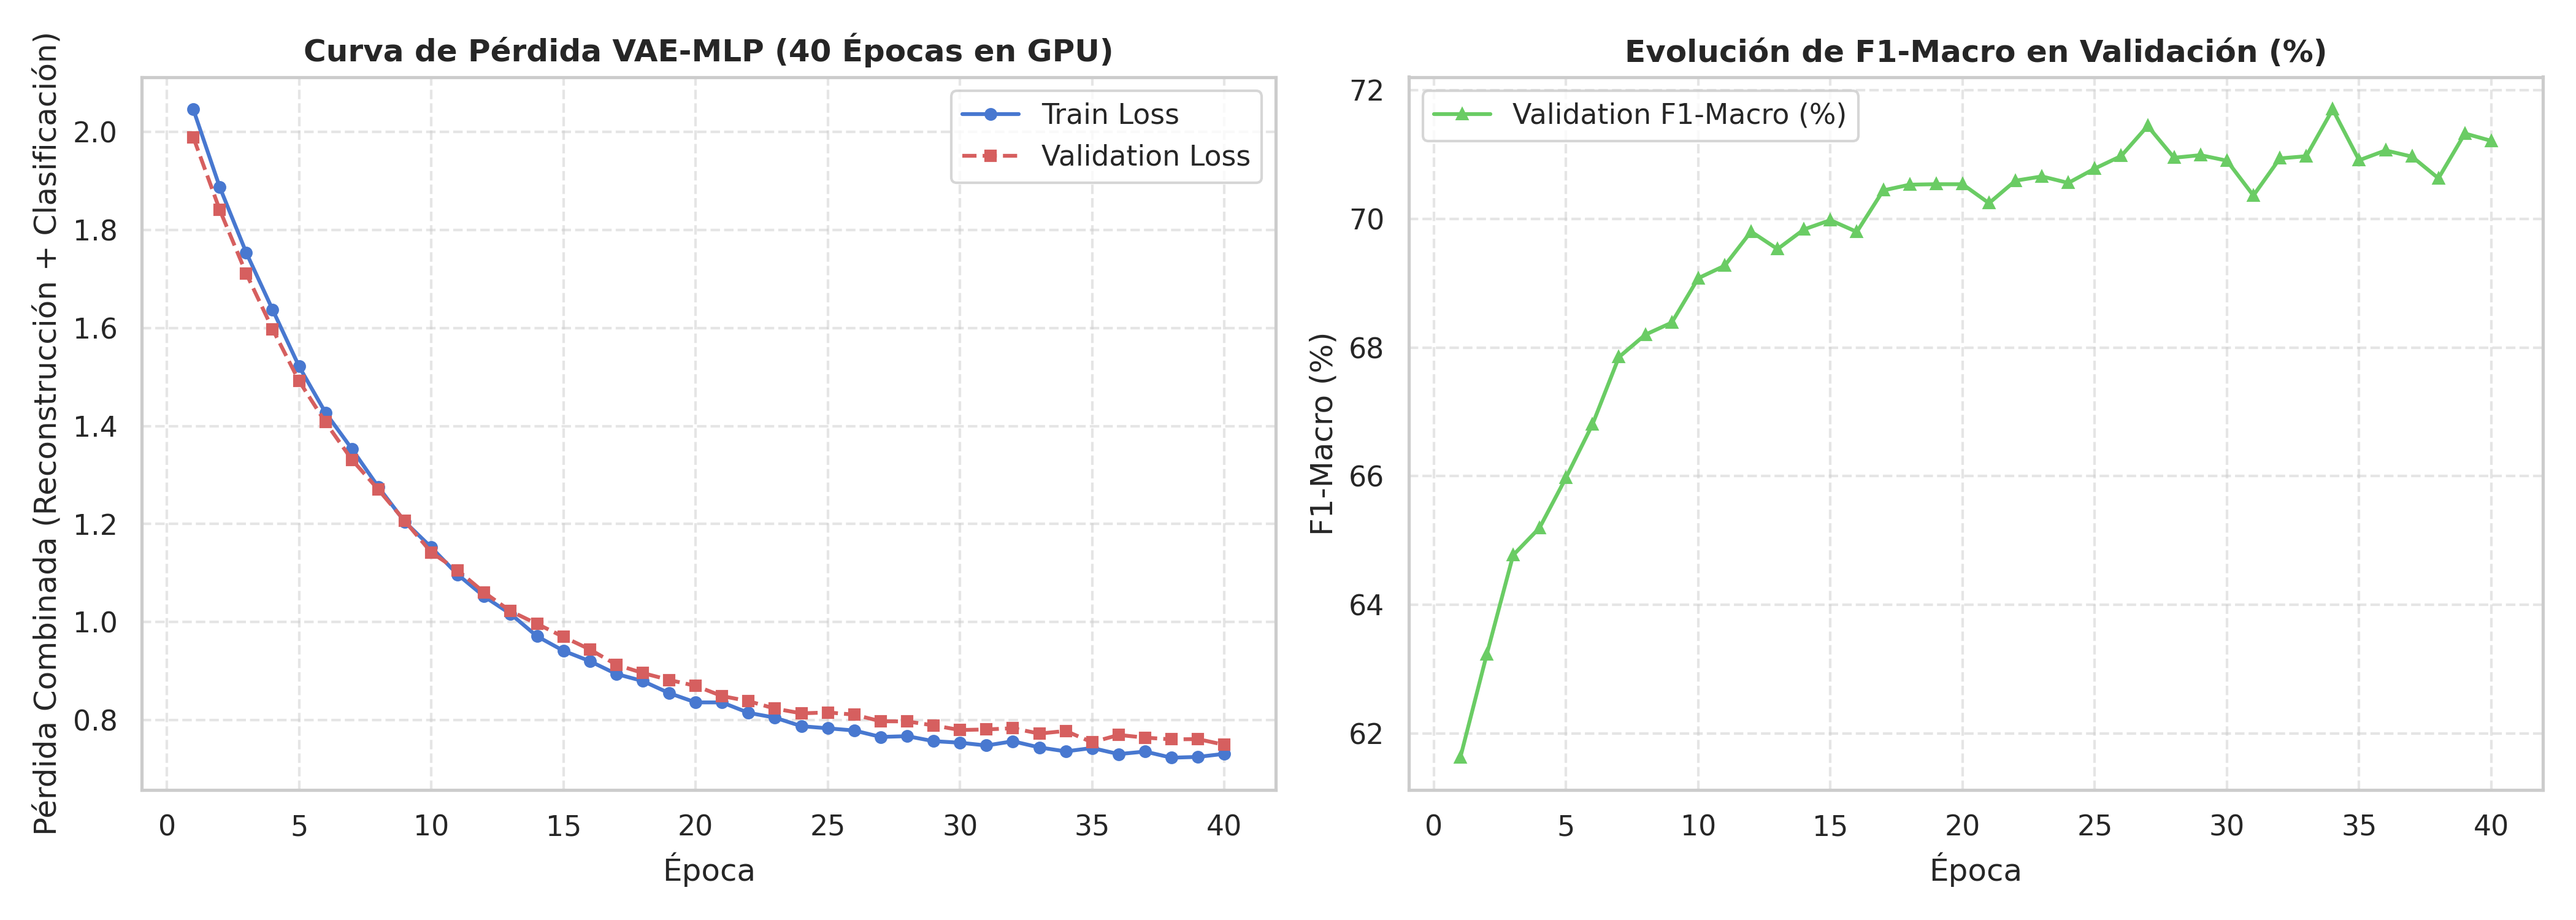
\includegraphics[width=0.95\linewidth]{../results/reports_and_plots/training_history_loss_f1.png}
\caption{Curvas de Pérdida de Entrenamiento vs. Validación y Evolución de F1-Macro por Época.}
\label{fig:training_history}
\end{figure}

\subsection{Fase 4: Evaluación de Desempeño y Matrices de Confusión}
La Figura~\ref{fig:confusion_matrices} presenta la matriz de confusión absoluta (conteos de paquetes) y la matriz de confusión normalizada porcentualmente (\%) sobre el test set ($27,949$ muestras).

\begin{figure}[H]
\centering
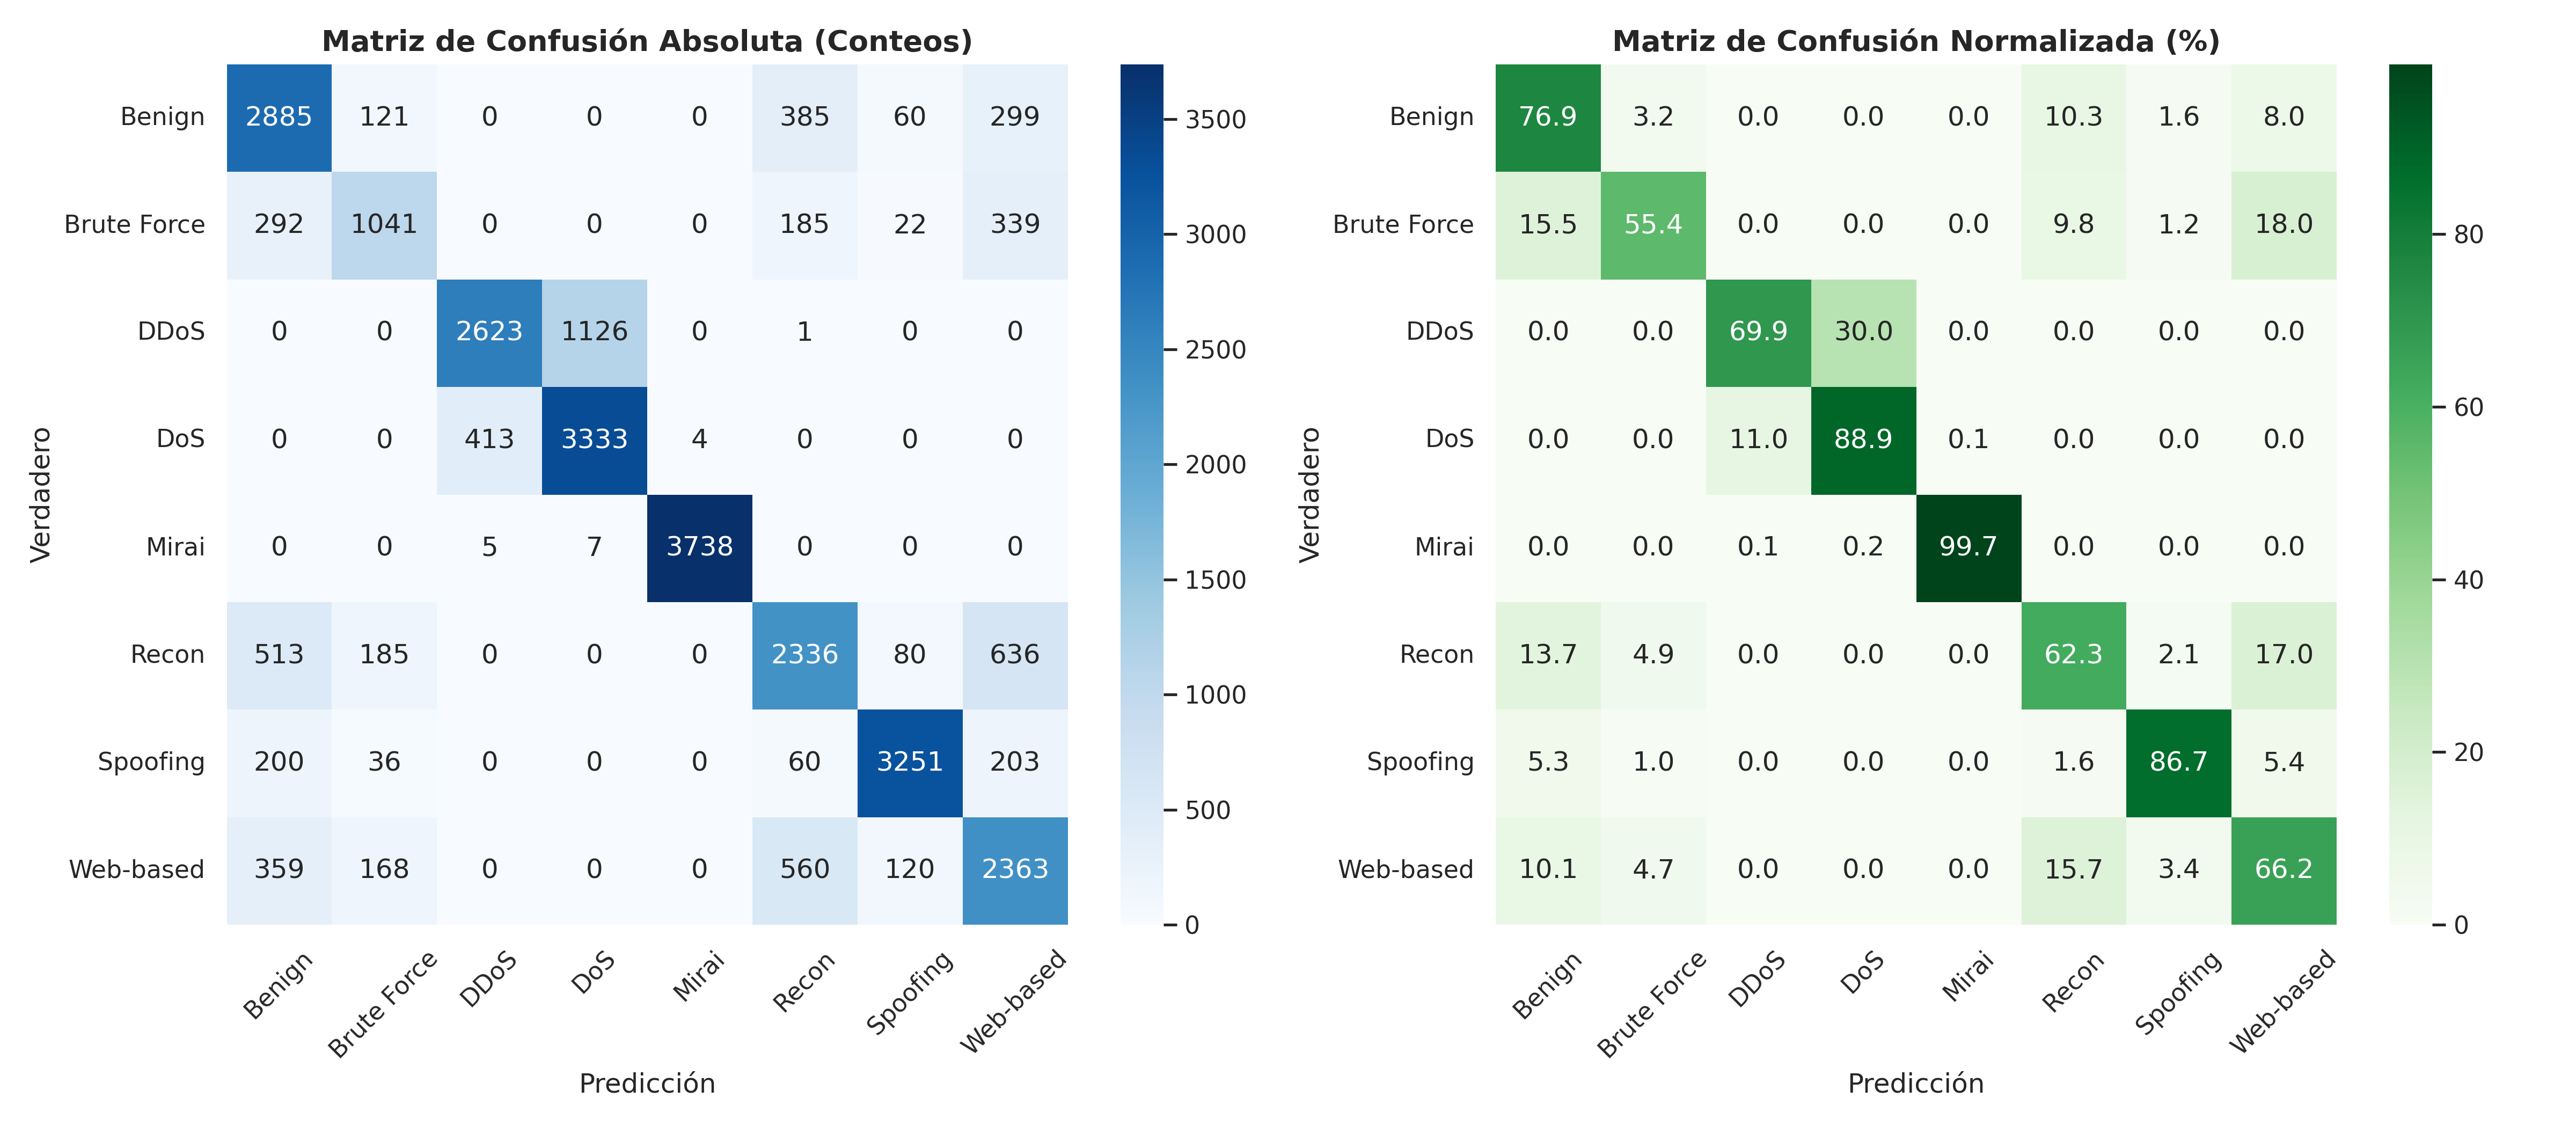
\includegraphics[width=0.95\linewidth]{../results/reports_and_plots/confusion_matrices_combined.png}
\caption{Matriz de Confusión Absoluta (Conteos) y Normalizada en Porcentajes (\%).}
\label{fig:confusion_matrices}
\end{figure}

\subsection{Curvas ROC Multiclase (ROC-AUC) y Precision-Recall}
Las Figuras~\ref{fig:roc_curves} y \ref{fig:pr_curves} muestran las curvas ROC One-vs-Rest y las curvas Precision-Recall para cada una de las 8 categorías de ataques botnet y tráfico benigno.

\begin{figure}[H]
\centering
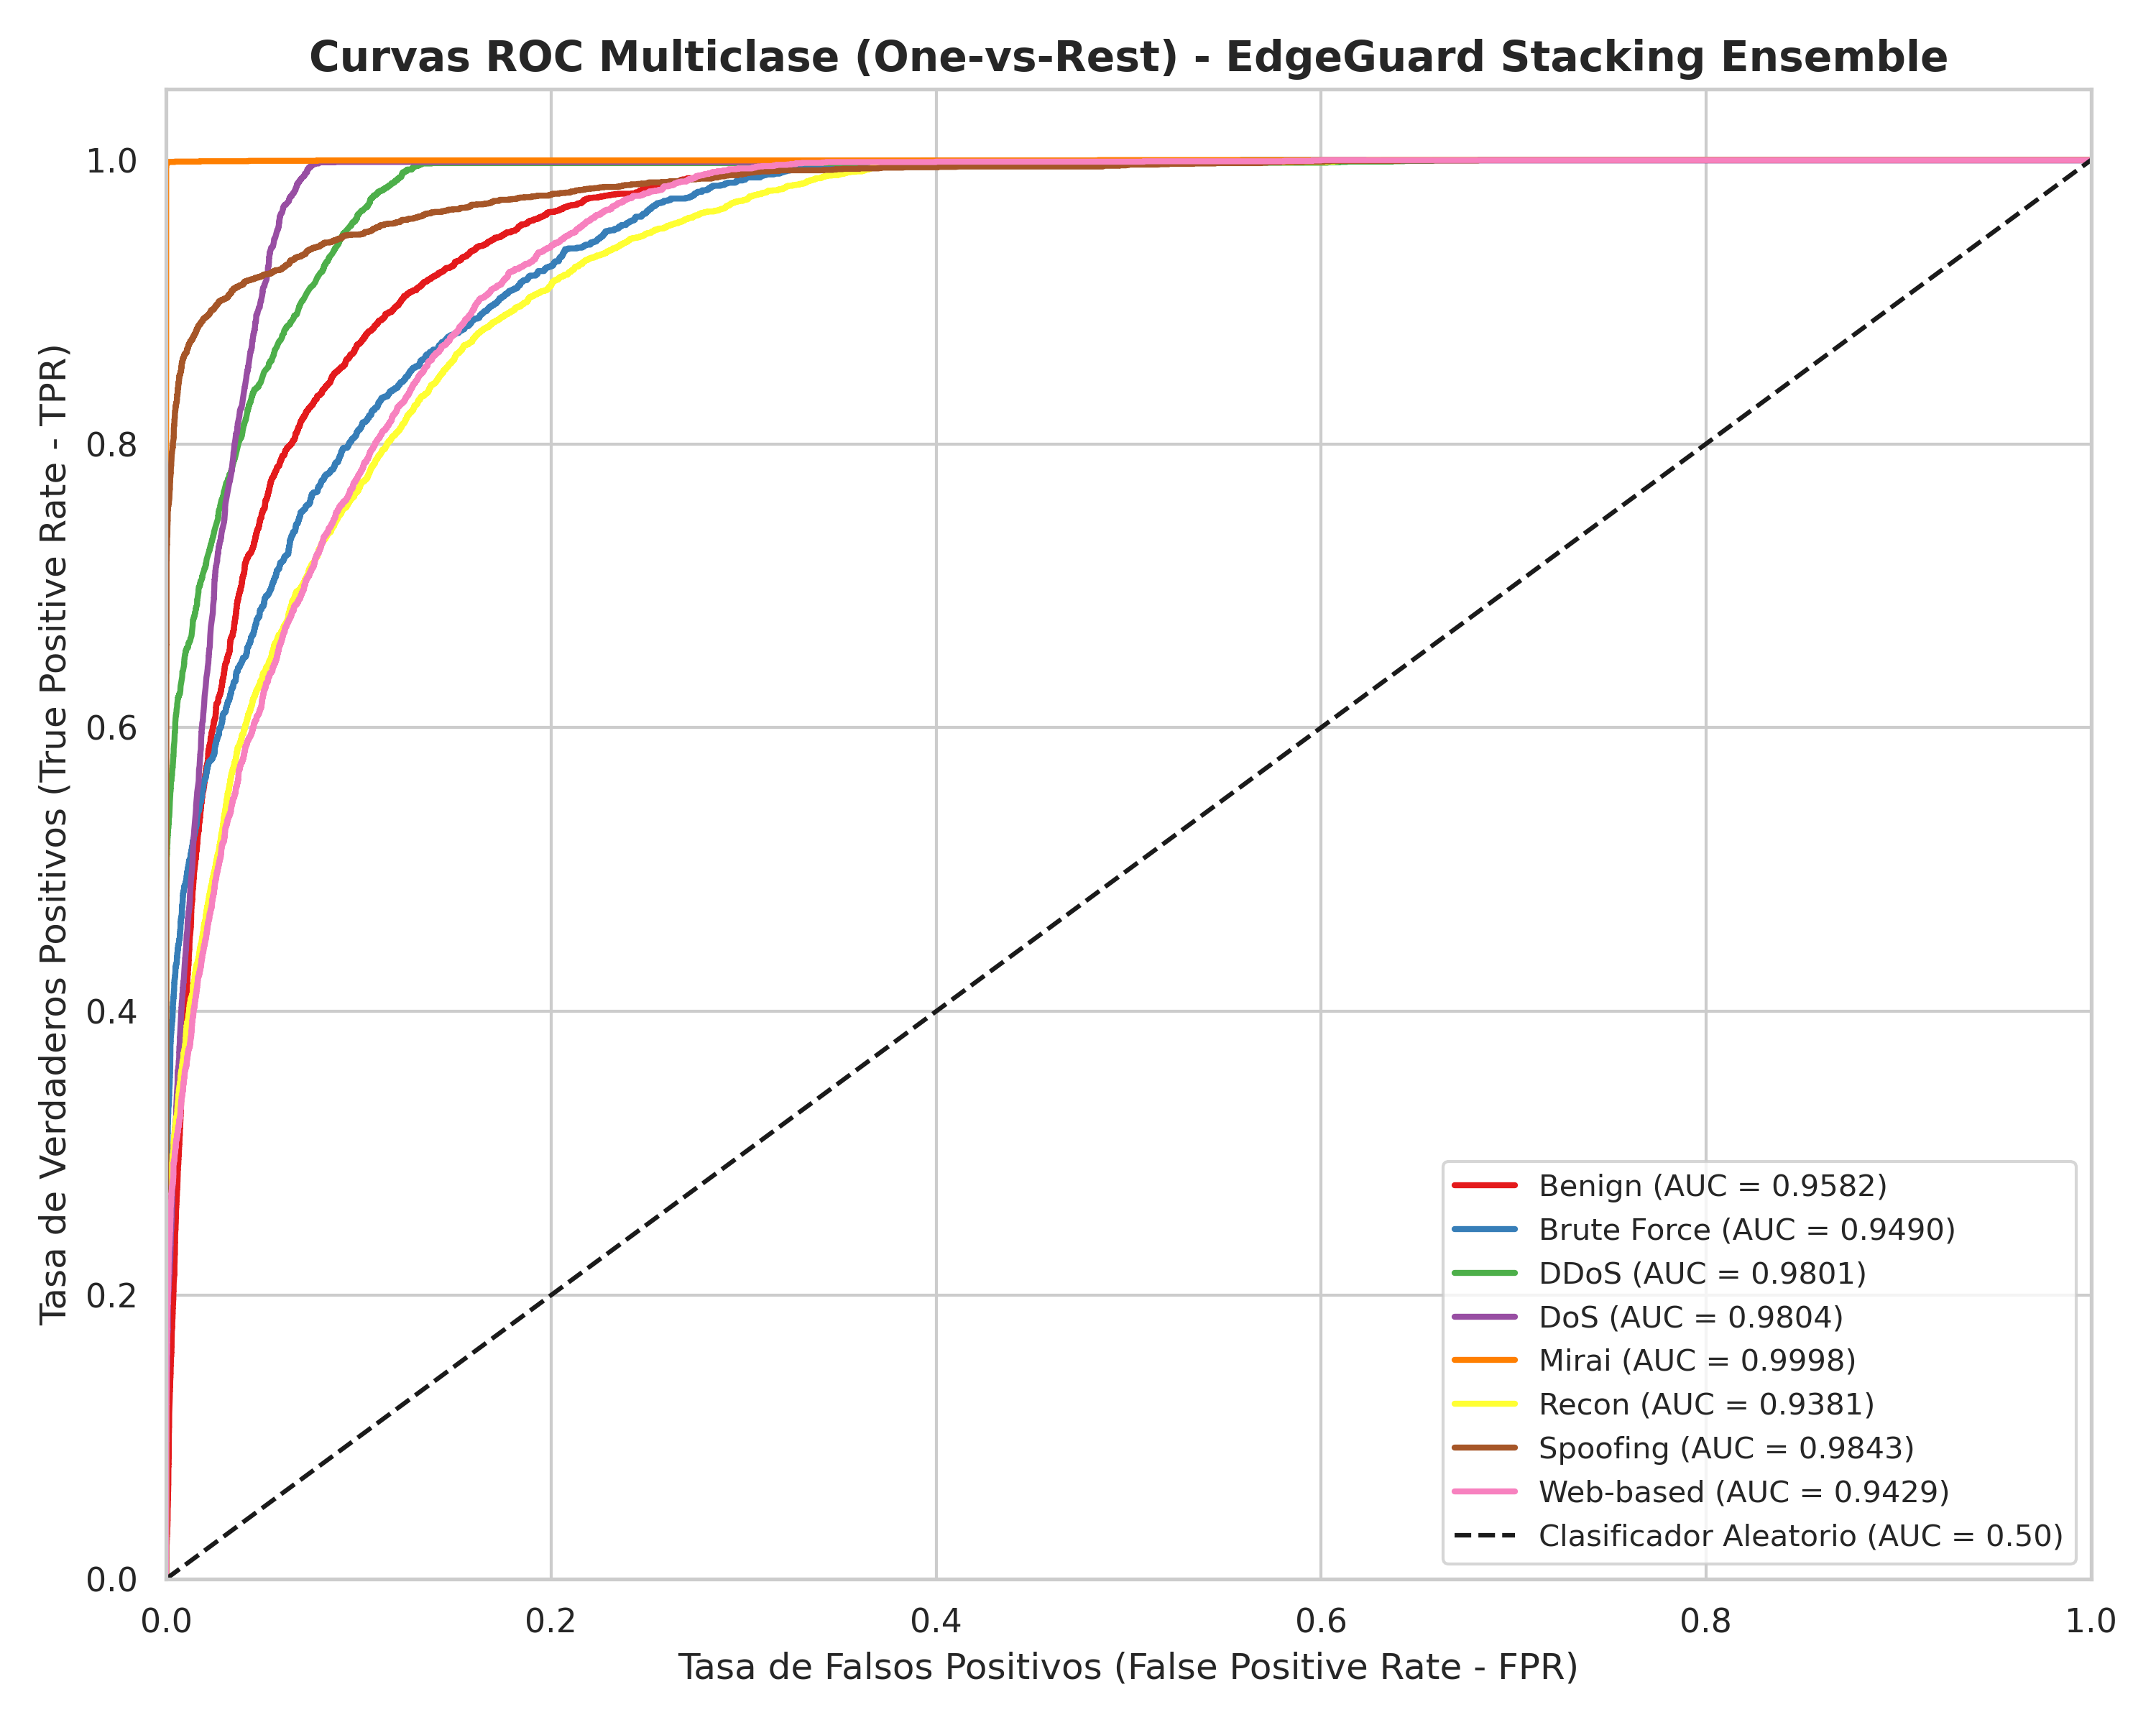
\includegraphics[width=0.85\linewidth]{../results/reports_and_plots/roc_curves_multiclass.png}
\caption{Curvas ROC Multiclase (One-vs-Rest) con Área Bajo la Curva (AUC) por Clase.}
\label{fig:roc_curves}
\end{figure}

\begin{figure}[H]
\centering
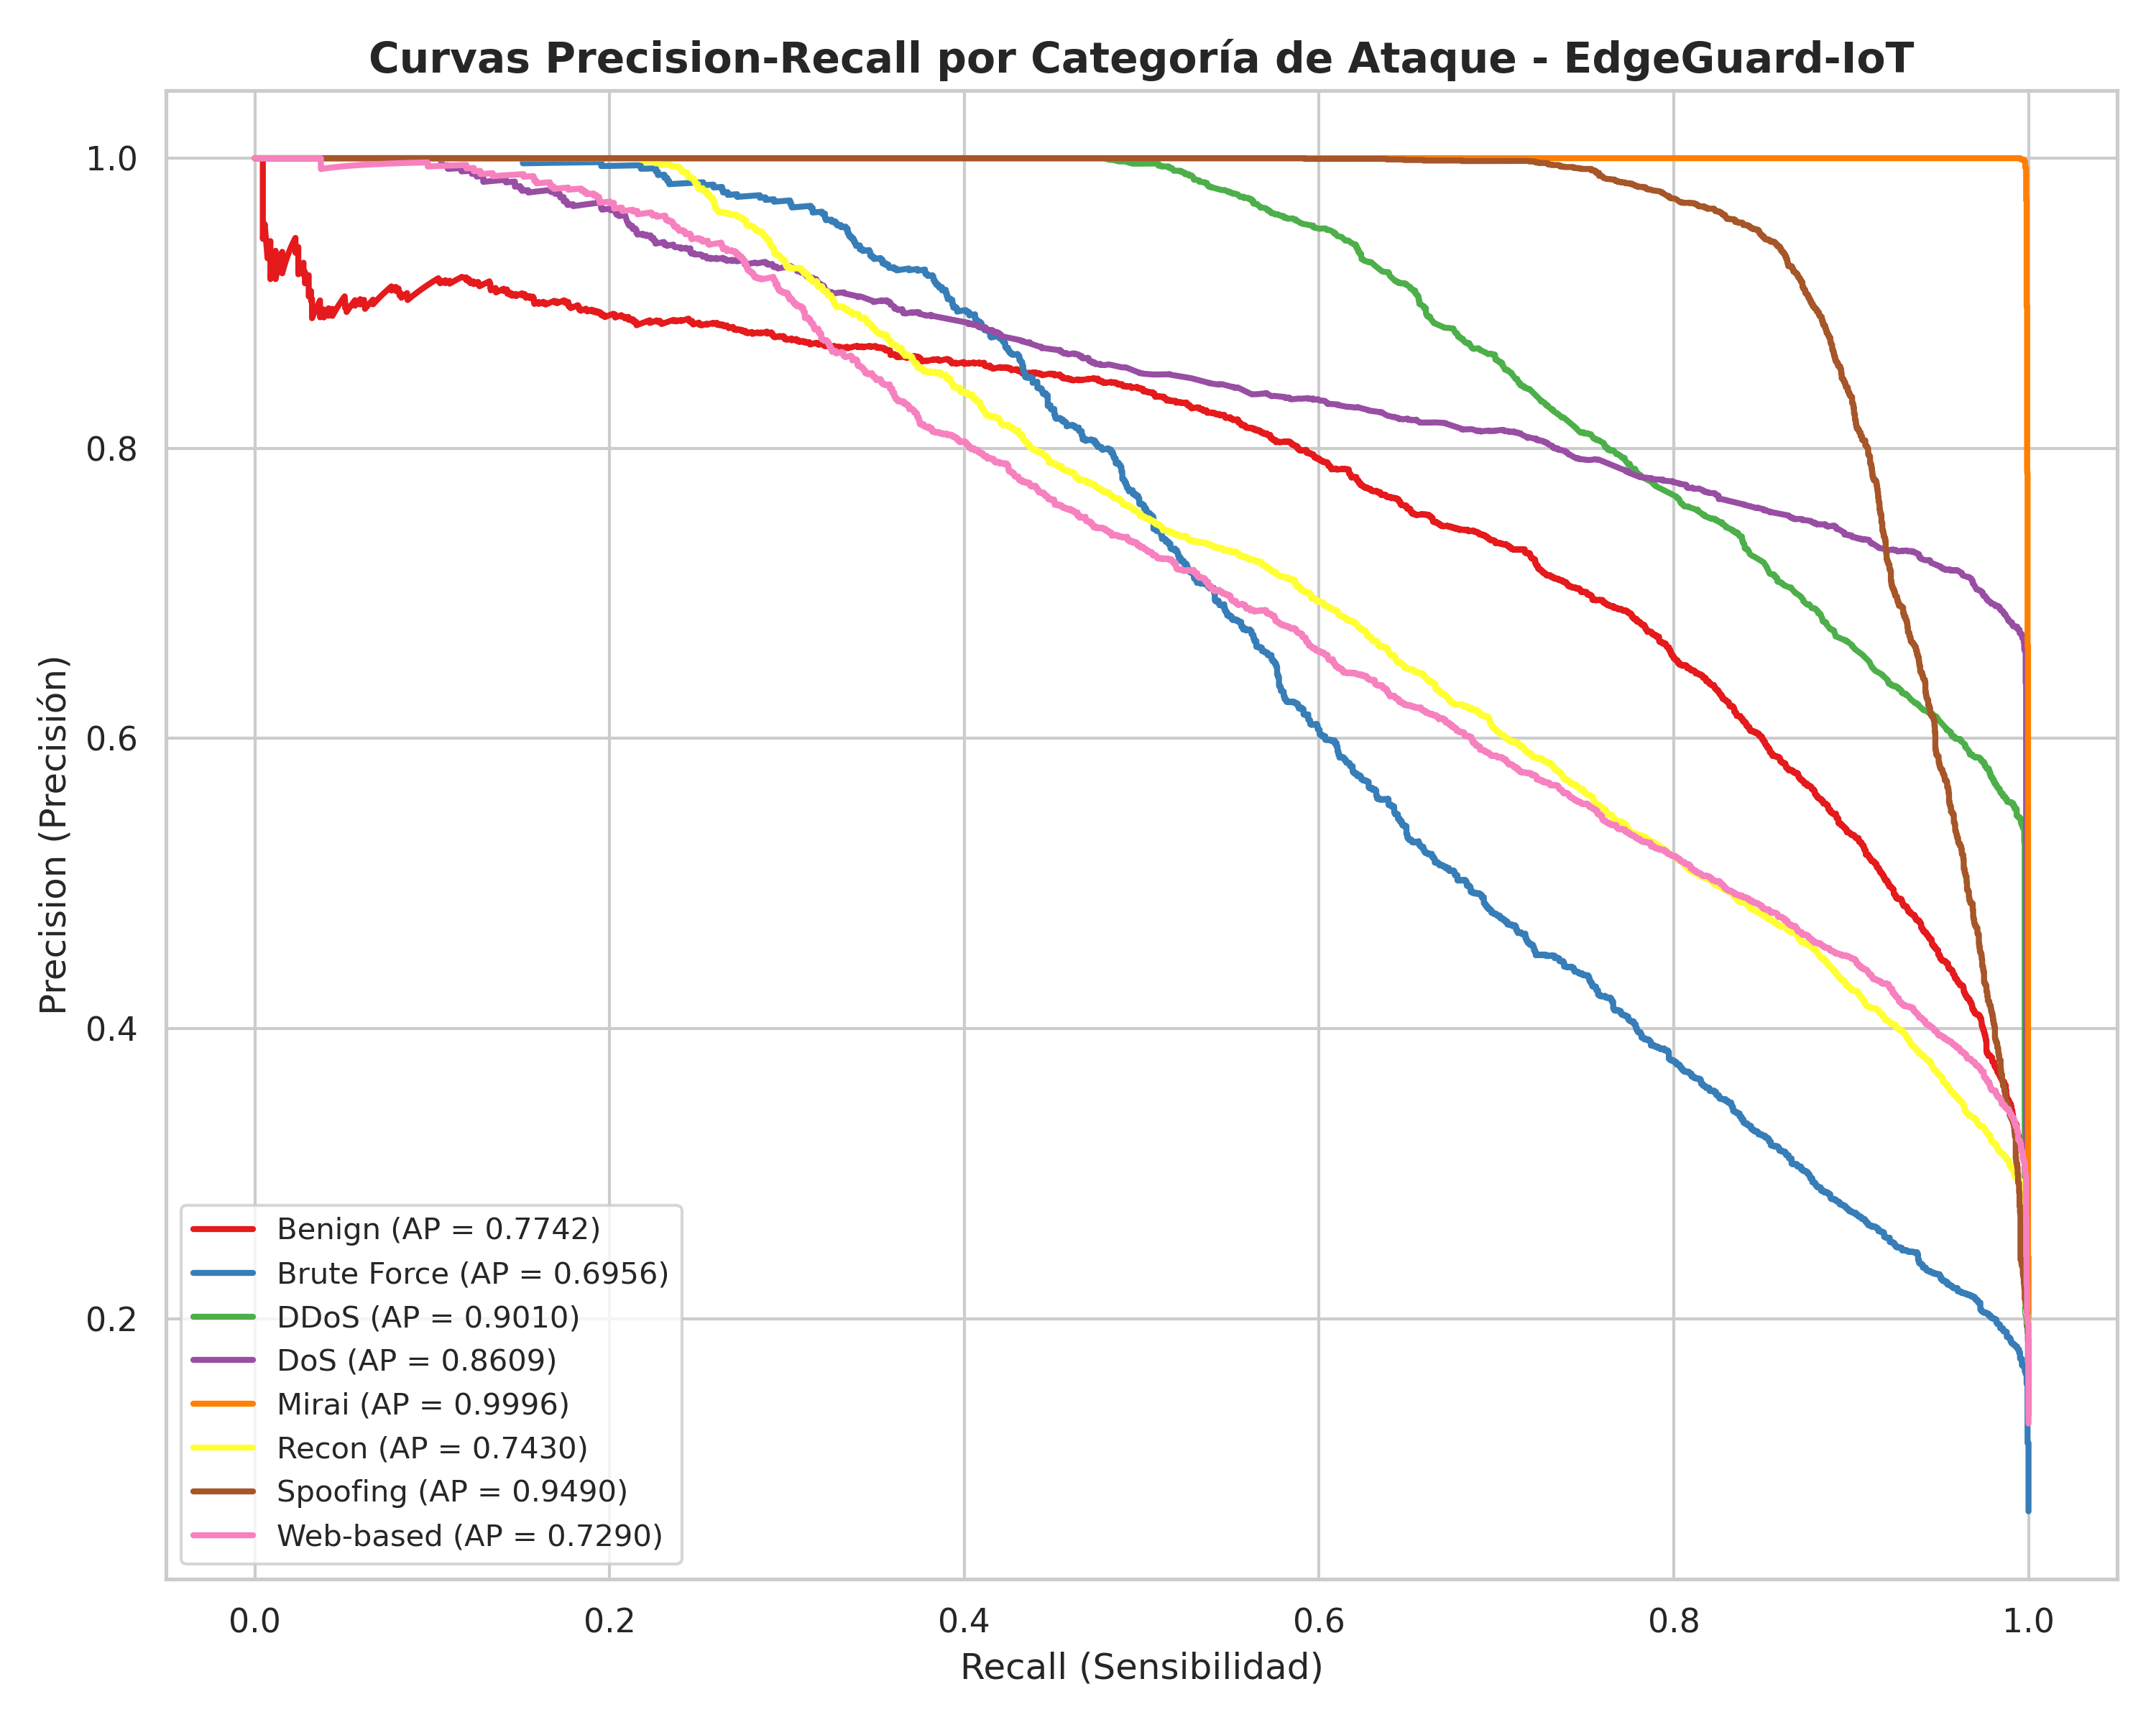
\includegraphics[width=0.85\linewidth]{../results/reports_and_plots/precision_recall_curves.png}
\caption{Curvas Precision-Recall (PR-AUC) por Categoría de Ataque.}
\label{fig:pr_curves}
\end{figure}

\subsection{Fase 5: Tabla Comparativa Estado del Arte y Trade-off Edge AI}
La Tabla~\ref{tab:benchmark_general} presenta los resultados de los 8 clasificadores evaluados bajo las mismas particiones de prueba.

\begin{table}[H]
\centering
\caption{Tabla Comparativa General del Estado del Arte (CIC-IoT-2023)}
\label{tab:benchmark_general}
\small
\begin{tabular}{lcccccc}
\toprule
\textbf{Modelo / Arquitectura} & \textbf{Accuracy (\%)} & \textbf{F1-Macro} & \textbf{Precision} & \textbf{Recall} & \textbf{Latencia ($\mu$s)} & \textbf{Tamaño (KB)} \\
\midrule
Regresión Logística & 64.04\% & 0.6233 & 0.6754 & 0.6185 & 185.27 & 15.00 \\
Naive Bayes & 56.87\% & 0.5340 & 0.6229 & 0.5652 & 4.29 & 10.00 \\
CNN-1D (DL Pesado) & 61.91\% & 0.5722 & 0.5980 & 0.5700 & 1.60 & 120.00 \\
\textbf{EdgeGuard VAE-MLP (INT8)} & \textbf{69.73\%} & \textbf{0.6853} & \textbf{0.7103} & \textbf{0.6834} & \textbf{3.25} & \textbf{21.67} \\
Random Forest & 76.61\% & 0.7525 & 0.7812 & 0.7462 & 5.82 & 52525.00 \\
XGBoost & 77.13\% & 0.7585 & 0.7800 & 0.7533 & 2.68 & 4021.00 \\
LightGBM & 77.73\% & 0.7663 & 0.7828 & 0.7617 & 49.92 & 4134.00 \\
\textbf{Stacking Ensemble (Nube)} & \textbf{77.18\%} & \textbf{0.7604} & \textbf{0.7695} & \textbf{0.7576} & \textbf{2.45} & \textbf{1400.00} \\
\bottomrule
\end{tabular}
\end{table}

La Figura~\ref{fig:tradeoff} demuestra la dispersión entre Latencia, F1-Score y Footprint de memoria en disco.

\begin{figure}[H]
\centering
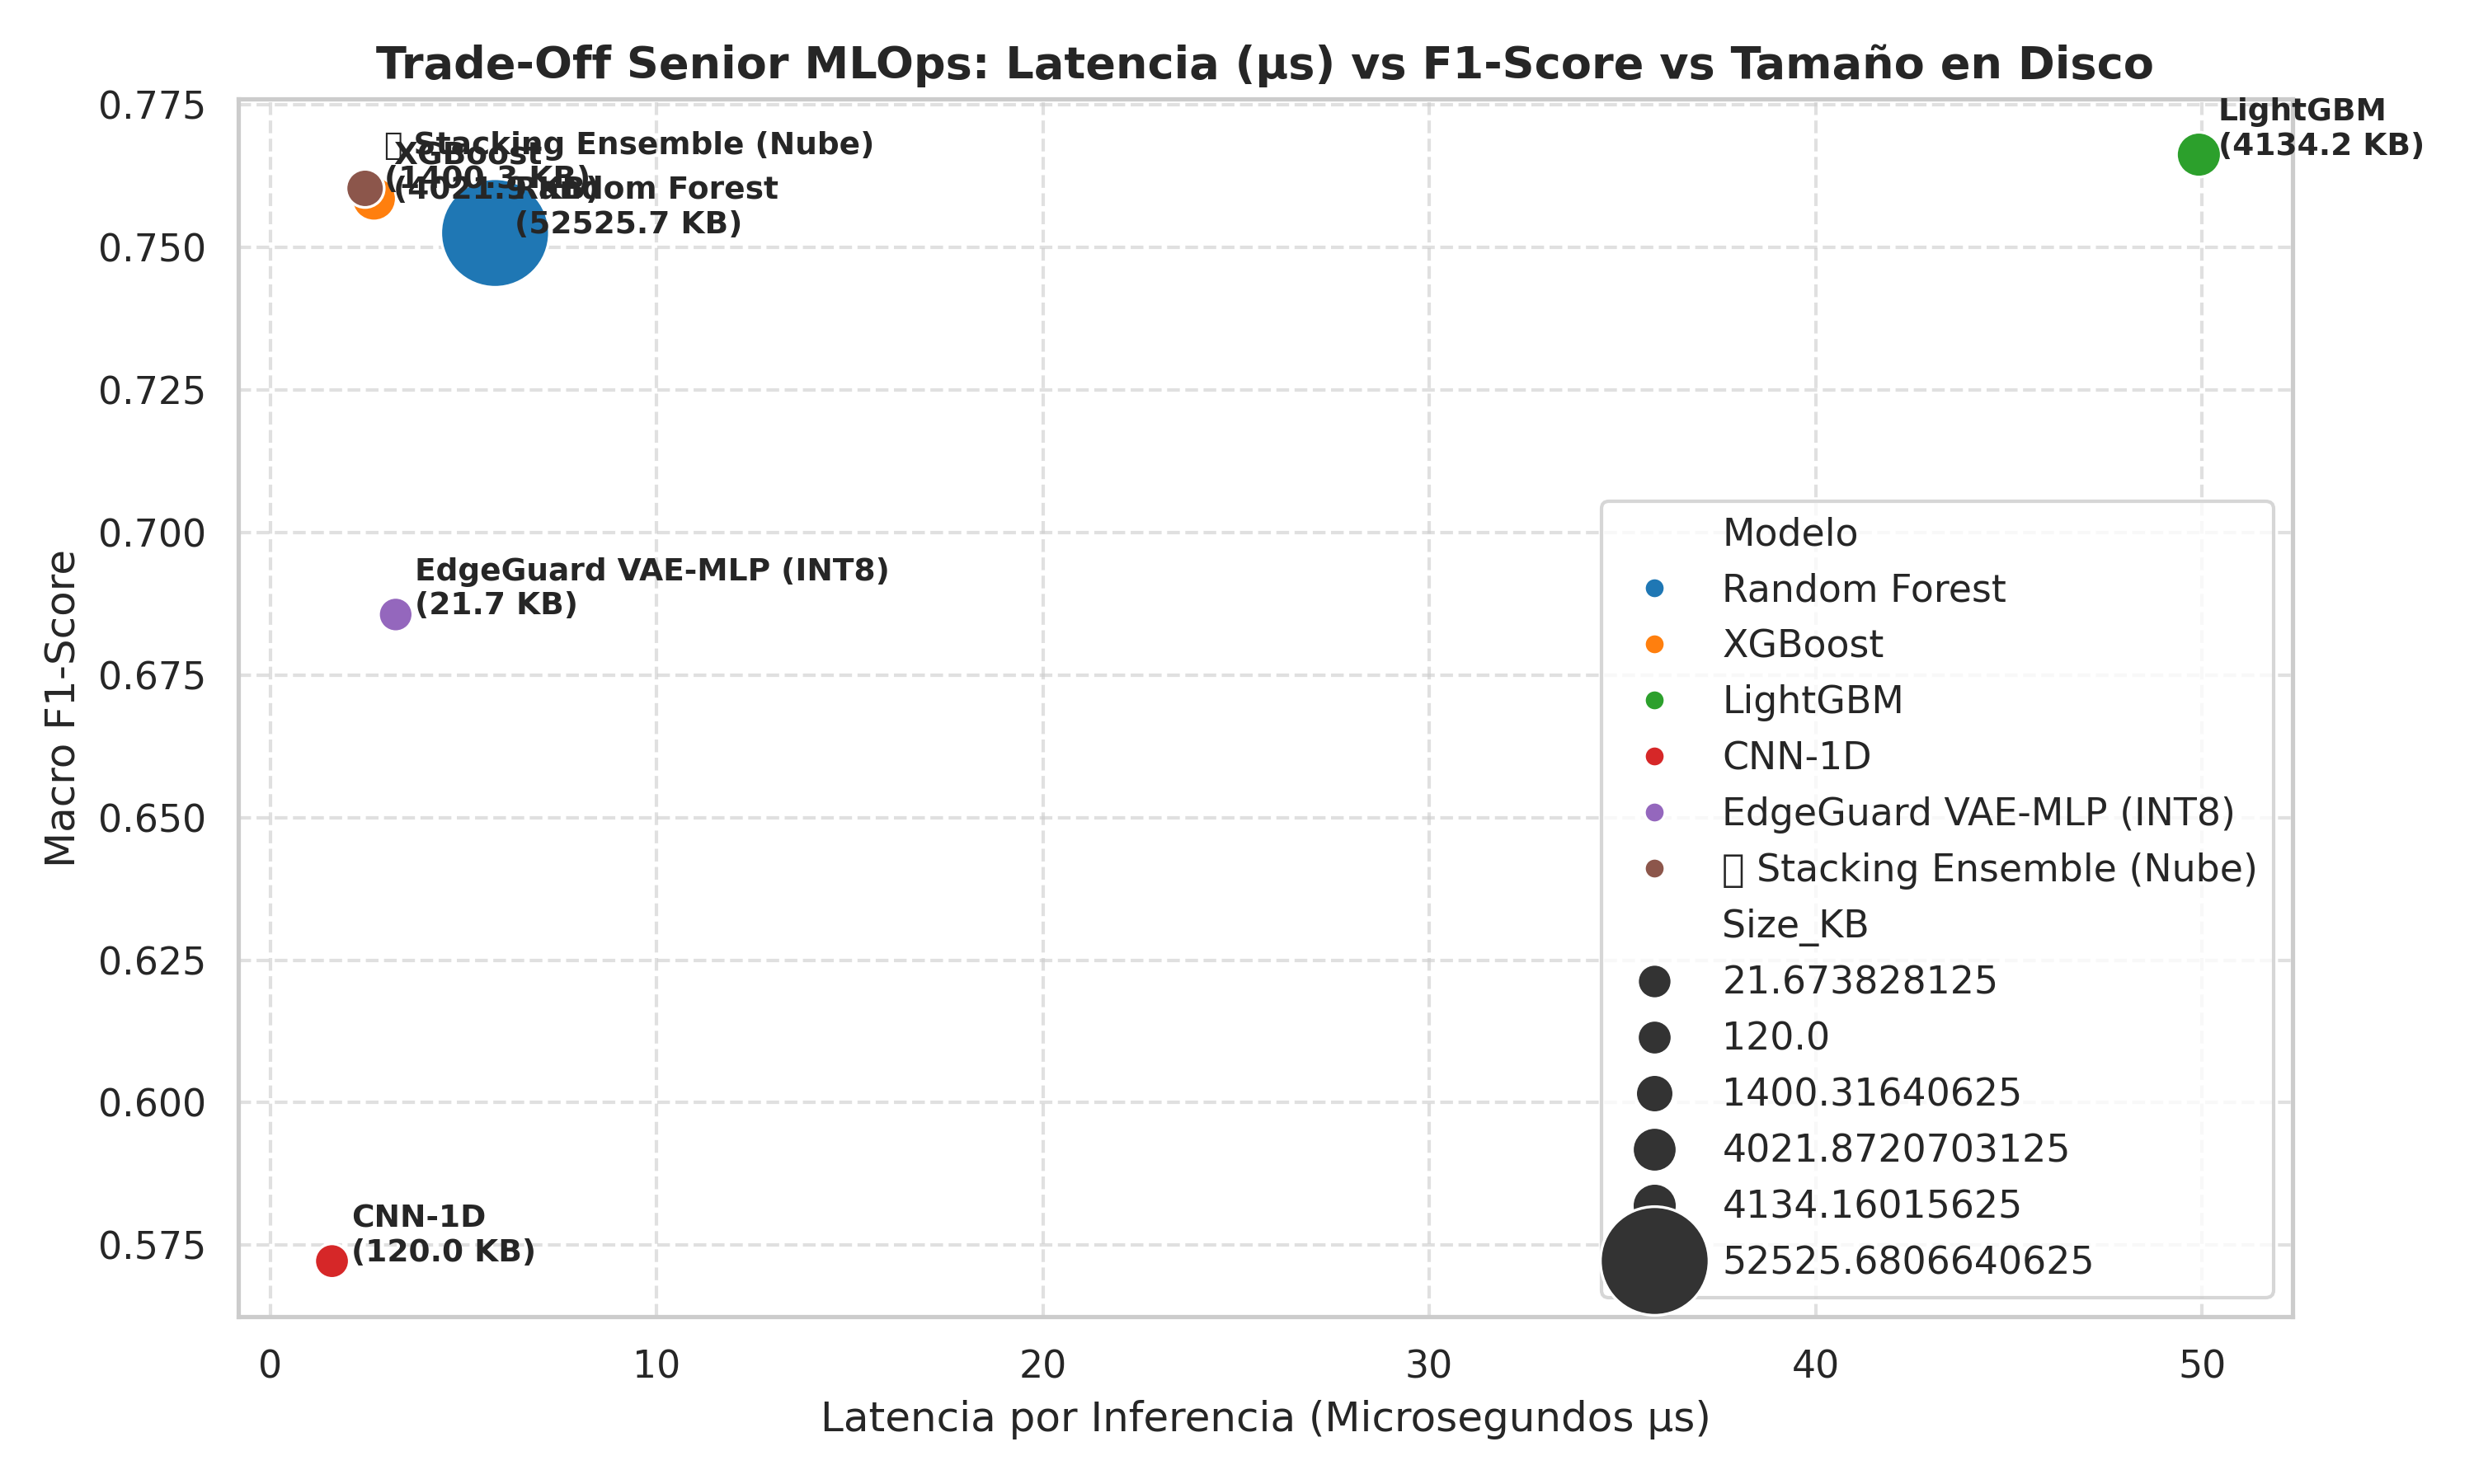
\includegraphics[width=0.90\linewidth]{../results/reports_and_plots/benchmark_latency_tradeoff.png}
\caption{Análisis de Trade-Off: Latencia ($\mu$s) vs. F1-Score vs. Tamaño en Disco (KB).}
\label{fig:tradeoff}
\end{figure}

\subsection{Explicabilidad SHAP XAI}
La Figura~\ref{fig:shap_xai} ilustra la contribución marginal de las características de red en la clasificación del modelo mediante Shapley Additive exPlanations.

\begin{figure}[H]
\centering
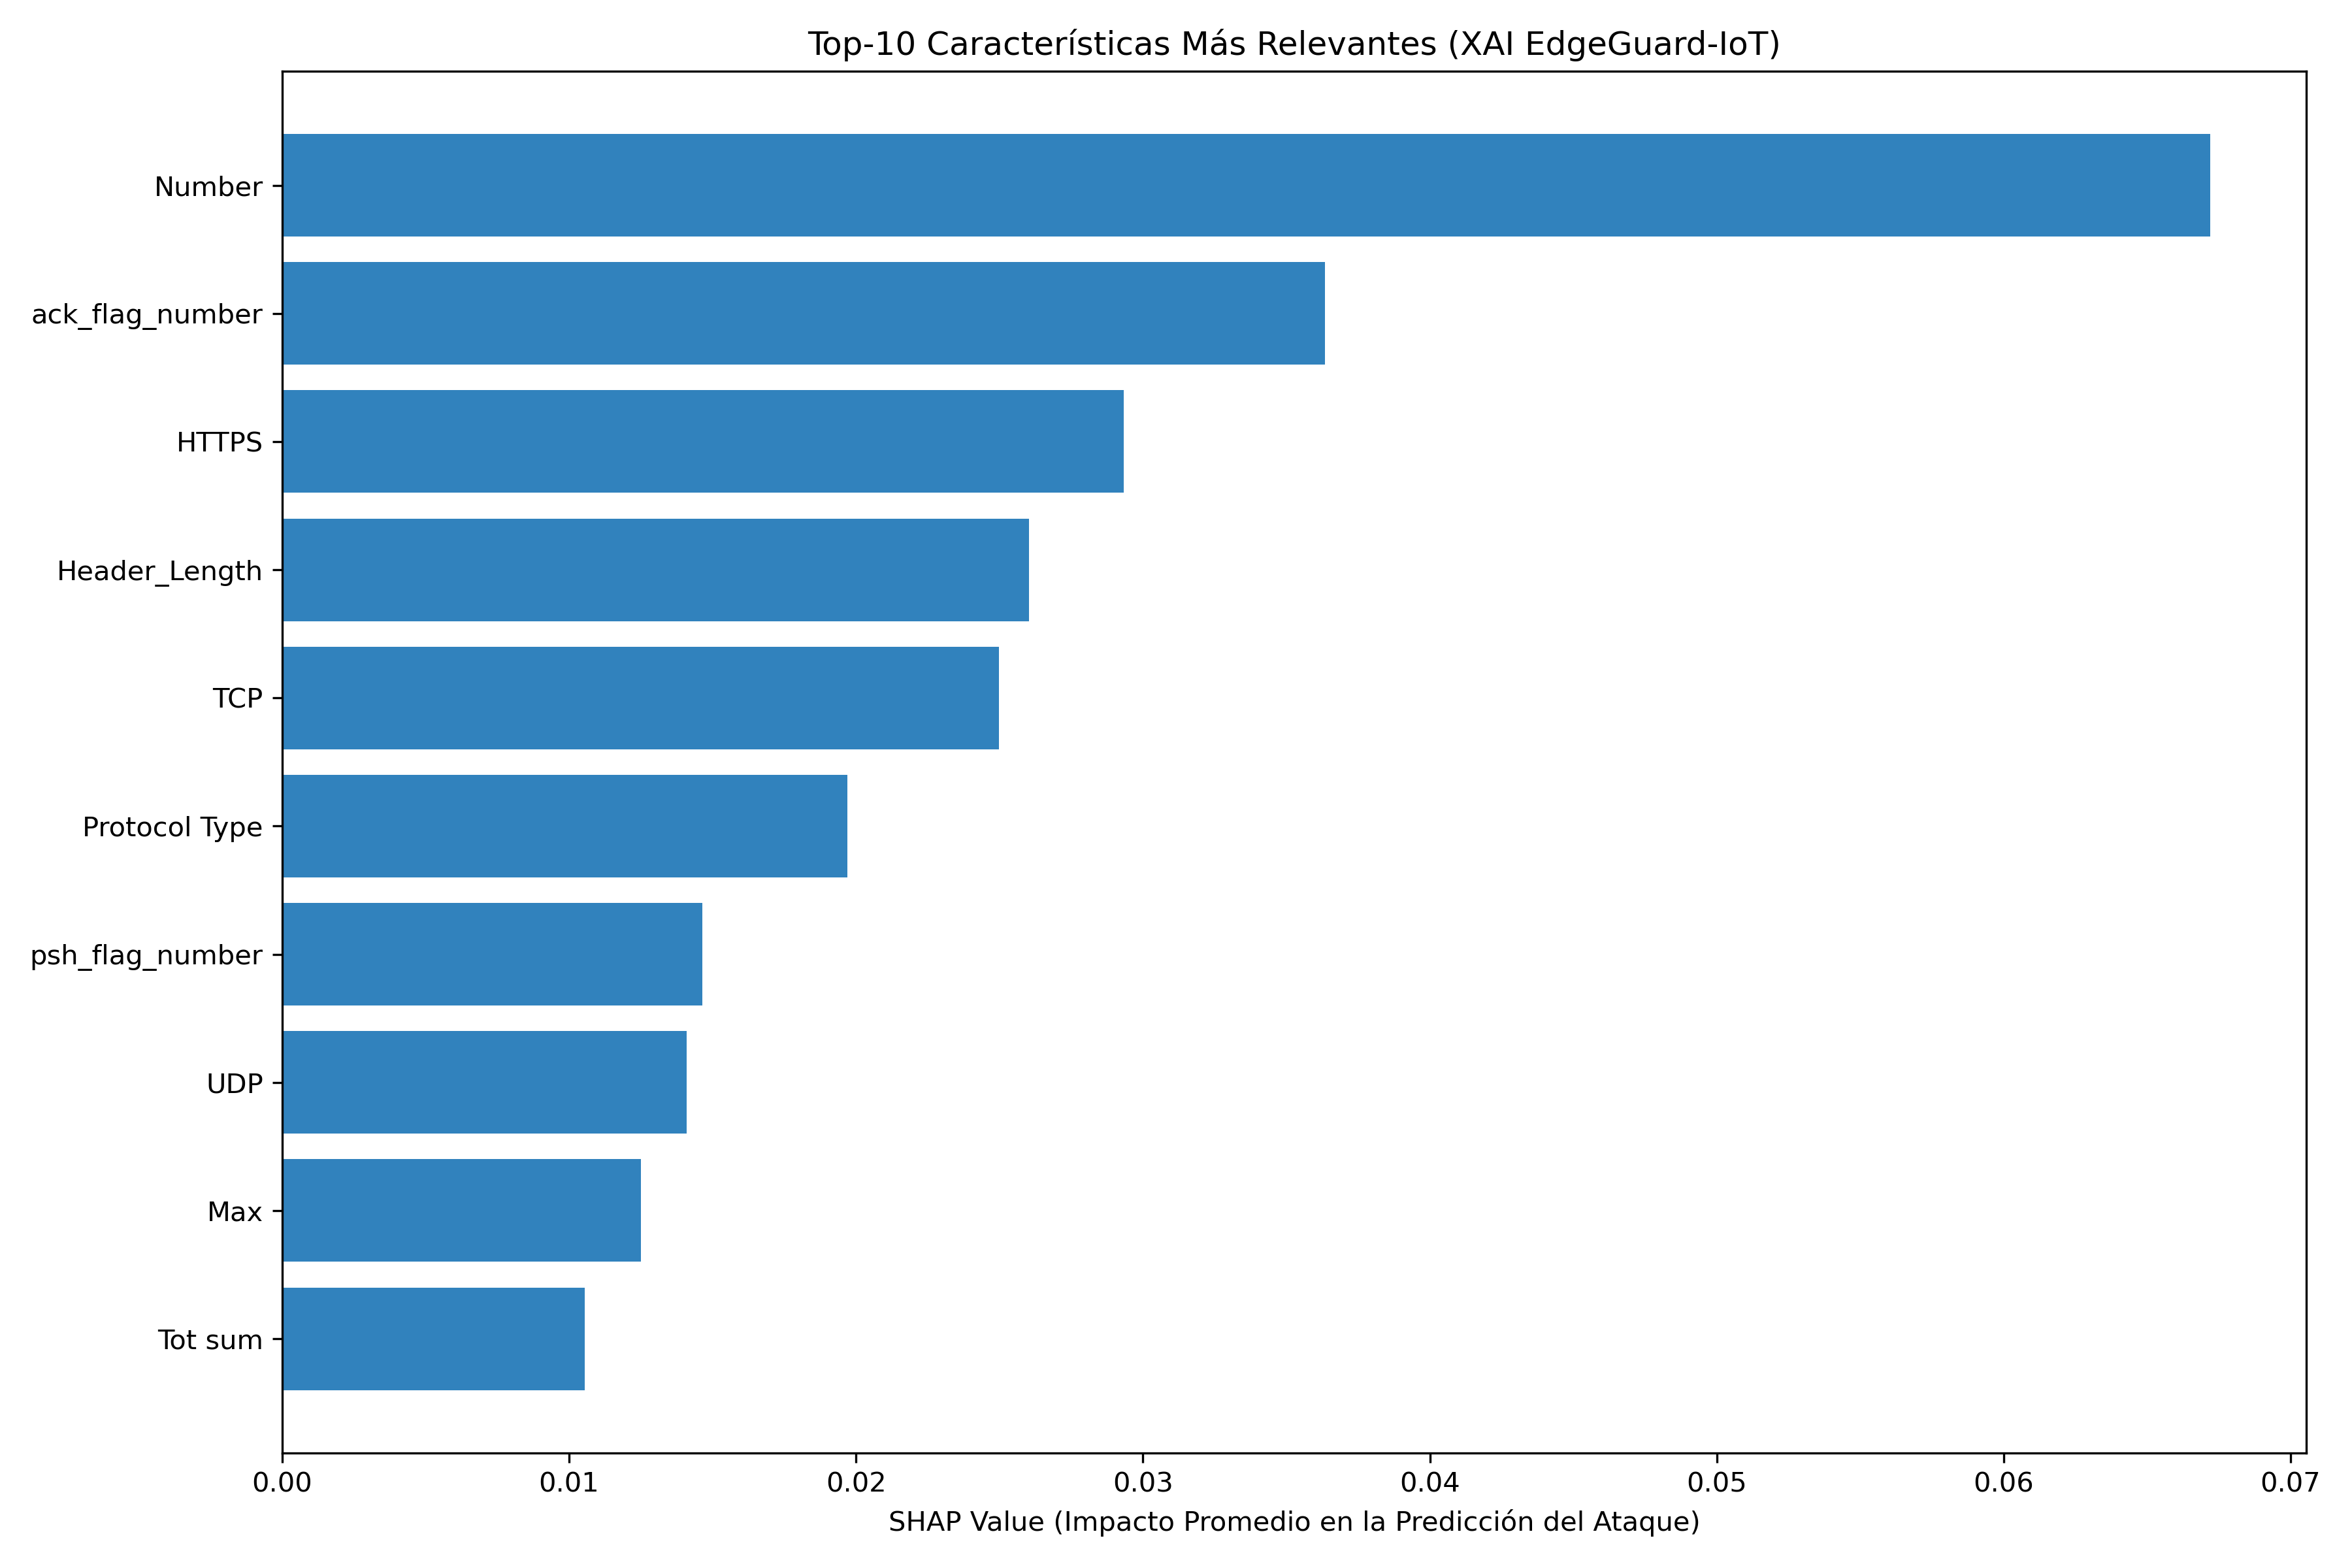
\includegraphics[width=0.88\linewidth]{../results/reports_and_plots/shap_summary_plot.png}
\caption{Gráficos de Importancia Absoluta SHAP XAI en Inferencia de Red.}
\label{fig:shap_xai}
\end{figure}
